\documentclass[12pt,a4paper]{article} 
\usepackage{a4wide}
\usepackage[utf8]{inputenc}
\usepackage{amsmath}
\usepackage{amsfonts}
\usepackage{amssymb}
\usepackage{graphicx}
\usepackage{float}
\usepackage[ngerman]{babel} 
\usepackage{pdflscape}
\usepackage{caption, booktabs}
\parindent0pt


\title{Teilentwurf von  LISE E-Learning System}

\author{Matthias Englert, Fabian Schilha, Andreas Rottach}
\date{Wintersemester 2014/2015}

\begin{document}
\maketitle
\newpage
\tableofcontents
\newpage

\section{Datenbankentwurf}

\subsection{Datebankdiagramm}
\begin{figure}[H]
	\centering
	\paragraph{Aufbau der Relationalen Datenbank}	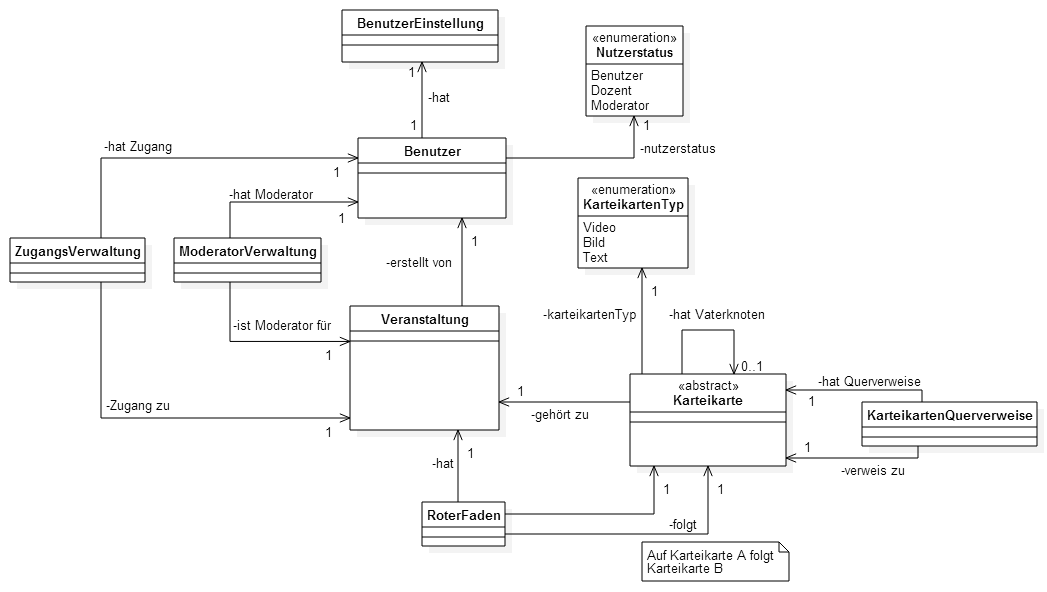
\includegraphics[width=\textwidth]{Bilder/Datenbank/Datenbankentwurf.png}
	\caption{Datenbankdiagramm}
	\label{Datenbankdiagramm}
\end{figure}

\subsection{Beschreibung der Tabellen}
\begin{tabular}{|lp{12cm}|}
\hline
TABELLE			&  Veranstaltung\\ 
BESCHREIBUNG	&  Speichert alle Veranstaltungen an der Universität Ulm\\ 
VERWALTET		&  Veranstaltungsinformationen und -einstellungen\\ 
SCHLÜSSEL		&  ID : Integer\\ 
\hline
&  \\ 
FELD		    &  Titel : String\\  
				&  \\
FELD		    &  Beschreibung : String\\ 
BESCHREIBUNG	&  Veranstaltungsbeschreibung\\
				&  \\
FELD		    &  Studiengang : Enum\\ 
BESCHREIBUNG	&  Veranstaltung ist bestimmten Studiengängen zugeordnet\\ 
				&  \\
FELD		    &  Semester : String\\ 
BESCHREIBUNG	&  Semsterinformationen werden im Format \glqq WS/SS JAHR\grqq gesichert \\
				&  \\
FELD		    &  Zugangspasswort : String\\ 
BESCHREIBUNG	&  speichert das verschlüsselte Passwort der Veranstaltung\\
				&  \\
FELD		    &  DisskusionErlaubt : Boolean\\ 
BESCHREIBUNG	&  True lässt Diskussionen zu, False deaktiviert diese Möglichkeit \\
				&  \\
FELD		    &  BewertungenErlaubt : Boolean\\ 
BESCHREIBUNG	&  True lässt Bewertungen zu, False deaktiviert diese Möglichkeit \\
				&  \\
FELD		    &  GruppenErlaubt : Boolean\\ 
BESCHREIBUNG	&  True lässt Gruppen zu, False deaktiviert diese Möglichkeit \\
				&  \\
FELD		    &  GruppenErlaubt : Boolean\\ 
BESCHREIBUNG	&  True lässt Gruppen zu, False deaktiviert diese Möglichkeit \\
				&  \\
FELD		    &  ModeratorKarteikartenBearbeiten : Boolean\\ 
BESCHREIBUNG	&  True Bearbeitungen von dem Moderator zu, False deaktiviert diese Möglichkeit. Dann kann er nur Diskussionen verwalten. \\
				&\\
FELD		    &  ModeratorKarteikartenBearbeiten : Boolean\\ 
BESCHREIBUNG	&  True Bearbeitungen von dem Moderator zu, False deaktiviert diese Möglichkeit. \\
				&\\
FELD		    &  Ersteller : Benutzer\\ 
BESCHREIBUNG	&  Fremdschlüssel, Verweis auf den Dozenten, der diese Veranstaltung erstellt hat. \\
\hline
\end{tabular}\\\\


\section{System-Architektur}

\subsection{Kommunikationsdiagramm}

\subsection{Klassendiagramm}

\begin{figure}[H]
	\centering
	\paragraph{Klassendiagramm}
	%	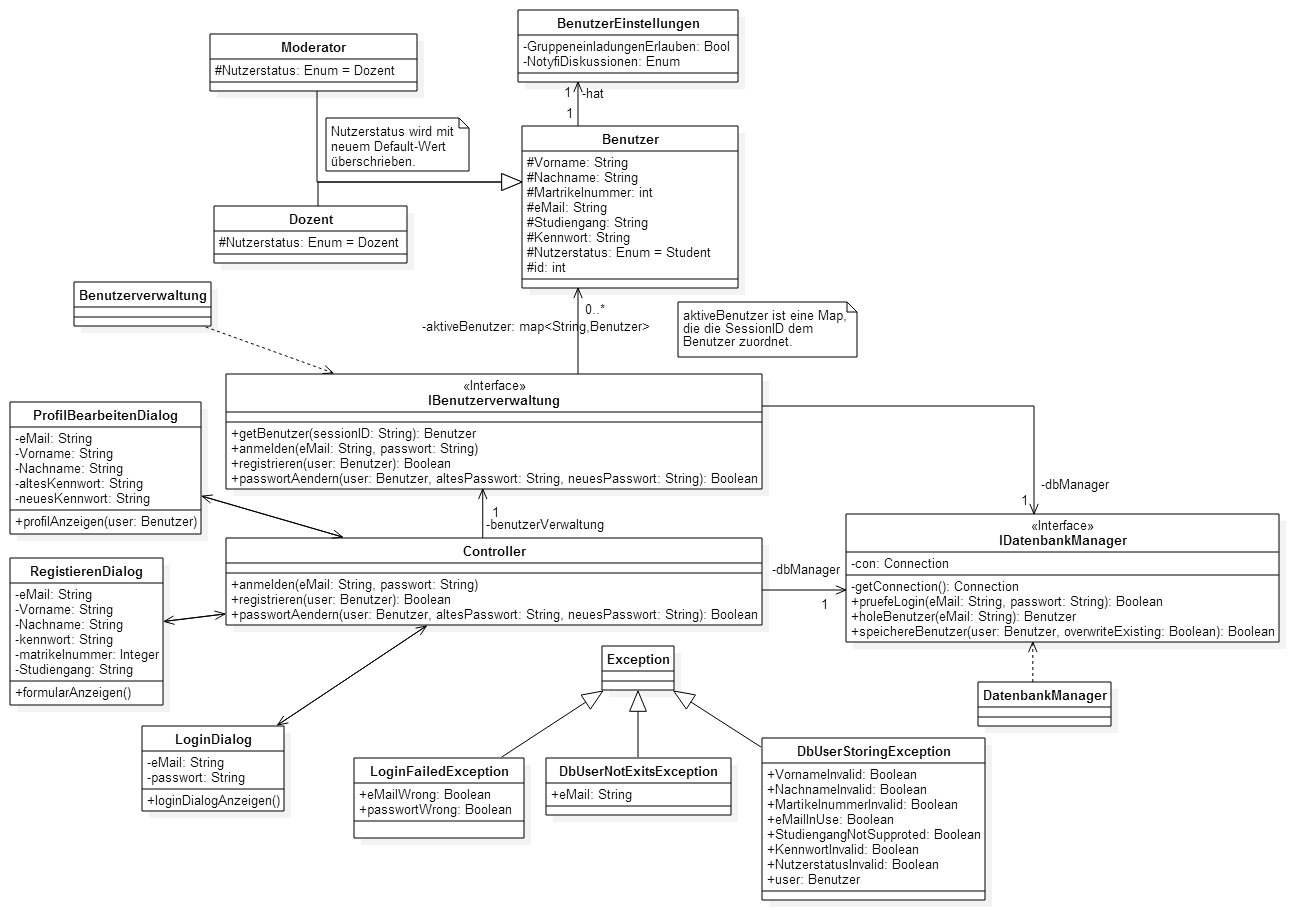
\includegraphics[width=\textwidth]{Bilder/Klassendiagramm/Klassendiagramm.png}
	\caption{Klassendiagramm}
	\label{Klassendiagramm des Teilsystems}
\end{figure}

\subsection{Methodenbeschreibung}


\begin{tabular}{|lp{12cm}|}
			\hline
			Operation &  \textbf{registrieren(neuerNutzer: Benutzer): Boolean }\\ 
			Beschreibung & Ein Benutzer registriert sich neu im System und gibt alle verlangten Daten an. Die Operation prüft ob die Daten korrekt sind und legt den neuen Benutzer gegebenenfalls an.\\ 
			Erzeugt &  Benutzer\\ 
			Pre &  Nutzer ist noch nicht registriert. \\ 
			Post & Nutzer ist im System angelegt.  \\ 
			\hline 
\end{tabular} \\\\



\end{document}
